\documentclass[11pt, a4paper]{article}

\usepackage{tikz}
\usepackage{amsmath}
\usepackage{placeins}
\usepackage{booktabs}

\begin{document}

\title{INDEPENDENT COMPONENT ANALYSIS}
\date{}
\maketitle

Independent Component Analysis is a statistical generative model which aims to reveal hidden independent additive components from multi-dimensional data.

\section{Mathematical Preliminaries}

\subsection{Single Random Variable}

Let the Probability Mass Function of a discrete random variable X be defined as follows.

\begin{table}[htbp]
	\centering
	\begin{tabular}{|c|c|c|c|c|}
		\toprule
		         & $x=1$ & $x=2$ & $x=3$ & $x=4$ \\
		\midrule
		$P(X=x)$ & 1/6   & 1/3   & 1/3   & 1/6   \\
		\hline
	\end{tabular}
\end{table}

The expectation $E(X)$ of this random variable is defined as follows.

\begin{align*}
	E(X) & = \sum_k x_k P(X=x_k)                                                                       \\
	     & = 1 \times \frac{1}{6} + 2 \times \frac{1}{3} + 3 \times \frac{1}{3} + 4 \times \frac{1}{6} \\
	     & = \frac{15}{6}                                                                              
\end{align*}

If a new variable $Y=2X+1$ is defined, the PMF of $Y$ becomes

\begin{table}[htbp]
	\centering
	\begin{tabular}{|c|c|c|c|c|}
		\toprule
		                & $y=2 \times 1  + 1$ & $y=2 \times 2  + 1$ & $y=2 \times 3  + 1$ & $y=2 \times 4  + 1$ \\
		\midrule
		$P(Y=y=2x + 1)$ & 1/6                 & 1/3                 & 1/3                 & 1/6                 \\
		\hline
	\end{tabular}
\end{table}

\begin{align*}
	E(Y) & = \sum_k y_k P(Y=y_k)         \\ 
	     & = \sum_k (2 x_k + 1) P(Y=y_k) \\
	     & = \sum_k (2x_k + 1) P(X=x_k)  \\
	     & = 2E(X) + 1                   
\end{align*}

Hence, expectation is a linear operator which satisfies $E(aX + b) = aE(X) + b$.

The variance of a discrete random variable $X$ is defined as

\begin{align*}
	Var(X) & = E((X-E(X))(X-E(X)))           \\
	       & = E(X^2 - 2E(X)X + E(X)E(X))    \\
	       & = E(X^2) - 2E(X)E(X) + E(X)E(X) \\
	       & = E(X^2) - E(X)^2               
\end{align*}

In case of continuous random variables, instead of Probability Mass Function a Probability Density Function is defined because the sample space is continuous and infinite as opposed to discrete and finite.

The expectation and variance of a continuous random variable are defined as

\begin{align*}
	E(X)   & = \int x P(X=x) dx            \\
	Var(X) & = \int (x - E(X))^2 P(X=x) dx 
\end{align*}

Just as in the case of discrete random variables where the sum of probabilities of all events in sample space must sum to 1, the area under PDF curve in the case of continuous random variable must also integrate to 1.

An example of a well known continuous random variable is the Gaussian random variable whose PDF is defined as follows.

\begin{align*}
	P(X=x) & = \frac{1}{\sqrt{2\pi\sigma^2}} e^{\frac{-(x-\mu)^2}{2\sigma^2}} \\
\end{align*}

with the following expectation and variance.

\begin{align*}
	E(X)   & = \mu      \\
	Var(X) & = \sigma^2 
\end{align*}

\subsection{A Pair of Random Variables}

Let the joint Probability Mass Function of a pair of discrete random variables X  and Y be defined as follows.

\begin{table}[htbp]
	\centering
	\begin{tabular}{|c|c|c|c|}
		\toprule
		P(X=x,\ Y=y) & $x=1$ & $x=2$ & $x=3$ \\
		\midrule
		$y=1$        & 3/8   & 3/16  & 3/16  \\
		$y=2$        & 1/8   & 1/16  & 1/16  \\
		\hline
	\end{tabular}
\end{table}

As usual, the sum of all probabilities is equal to 1. 

Given the joint distribution of a set of random variables, one can also find out the distribution of a subset of those random variables and the distribution of such a subset is called the marginal distribution. In the above example, the marginal distribution of $X$ and $Y$can be computed by summing up each column and row respectively in the table above.

\begin{align*}
	P(X=x_k) = \sum_{y_l} P(X=x_k,\ y=y_l) \\
	P(Y=y_k) = \sum_{x_l} P(X=x_l,\ y=y_k) \\	
\end{align*}

In the case of a pair of continuous random variables, their joint Probability Distribution Function becomes a surface in three dimensions. The marginal distributions take the following formulae.

\begin{align*}
	P(X=x) = \int_y P(X=x,\ y=y)dy \\
	P(Y=y) = \int_x P(X=x,\ y=y)dx \\
\end{align*}

Two random variables are said to statistically independent if and only if

\begin{align*}
	P(X=x,\ Y=y) = P(X=x)P(Y=y) 
\end{align*}

For independent random variables, the following result holds.

\begin{align*}
	E(f(X)g(Y)) & = \int \int f(x)g(y)P(X=x,\ Y=y)dxdy      \\ 
	            & = \int \int f(x)g(y) P(X=x) P(Y=y) dxdy   \\
	            & = \int f(x) P(X=x) dx \int g(y) P(Y=y) dy \\
	            & = E(f(X))E(g(Y))                          
\end{align*}

A weaker form of independence is uncorrelatedness. If $f(X)$ and $g(Y)$ are defined such that $f(X)=X$ and $g(Y) = Y$ and $E(XY) = E(X)E(Y)$ holds true, then two variables are said to be uncorrelated.

\subsection {Sum of Random Variables}

If $X$ denotes the outcome of roll of a dice and $Y$ denotes the outcome of roll of another dice, then $Z=X+Y$ denotes a random variable whose value is equal to the sum of the two rolls. If PMFs of $X$ and $Y$ are known, what is the PMF of $Z=X+Y$?

\begin{align*}
	P(Z=X+Y=z) & = \sum_x P(X=x,\ Y=z-x) \\
	           & = \sum_y P(X=z-y,\ Y=y) 
\end{align*}

It is easy to see why the above equation holds. To find $P(Z=z)$, one has to sum the probabilities $P(X=x,\ Y=y)$ of all possible scenarios where $x+y=z$. In the case of continuous random variables the formulae become

\begin{align*}
	P(Z=X+Y=z) & = \int P(X=x,\ Y=z-x) dx \\
	           & = \int P(X=z-y,\ Y=y) dy 
\end{align*}

Random variable sums are commutative and associative.

\begin{align*}
	X + Y     & = Y + Z       \\
	X + Y + Z & = (X + Y) + Z \\
	          & = X + (Y + Z) 
\end{align*}

The expectation of a sum of two random variables is the sum of expectations of individual random variables.

\begin{align*}
	E(X+Y) & = \int \int (x+y)P(X=x,\ Y=y)dxdy                                     \\
	       & = \int \int xP(X=x,\ Y=y)dxdy + \int yP(X=x,\ Y=y)dxdy                \\
	       & = \int x\ \int P(X=x,\ Y=y) dy\ dx + \int y\ \int P(X=x,\ Y=y) dx\ dy \\
	       & = \int xP(X=x)dx + \int yP(Y=y)dy                                     \\
	       & = E(X) + E(Y)                                                         
\end{align*}

Interestingly, If $X$ and $Y$ are independent Gaussian random variables then the above result holds for variances too.

\begin{align*}
	E(X+Y)   & = E(X) + E(Y)     \\
	Var(X+Y) & = Var(X) + Var(Y) 
\end{align*}

\section{Motivation}

Suppose there are $N$ people speaking at a party and there are $N$ microphones placed at different locations recording sound. Each microphone is recording a simultaneous mix of all speakers' sounds depending on the relative position of the microphone from the speakers. Looking at the microphone recordings alone, is it possible to decipher what each speaker said? 

\section{Problem Statement}

Denote each speaker's sound as a random variable $S_i$ (S stands for signal). A square mixing matrix $A$ is assumed to be responsible for linearly transforming $N$ signals into another set of $N$ random variables observed one each by a microphone.  

\begin{align*}
	\begin{pmatrix} 
	X_1 \\ 
	X_2 \\ 
	. \\ 
	. \\ 
	. \\ 
	X_N 
	\end{pmatrix} &=
	\begin{pmatrix} 
	a_{11} & a_{12} & ... & a_{1N} \\ 
	a_{21} & a_{22} & ... & a_{2N} \\ 
	.      & .      & ... & .      \\
	.      & .      & ... & .      \\
	.      & .      & ... & .      \\ 
	a_{N1} & a_{N2} & ... & a_{NN} \\ 
	\end{pmatrix}
	\begin{pmatrix} 
	S_1 \\ 
	S_2 \\ 
	. \\ 
	. \\ 
	. \\ 
	S_N 
	\end{pmatrix} \\
	\\
	\boldsymbol{X} &= A \boldsymbol{S}
\end{align*}

If the $j$th column of the matrix $A$ is denoted by $\boldsymbol{a_j}$, then the equation becomes

\begin{align*}
	\boldsymbol{X} = \sum_j \boldsymbol{a_j} S_j 
\end{align*}

A set of observations corresponding to $\boldsymbol{X}$ are given and the goal is to recover $\boldsymbol{S}$.

\begin{align*}
	\boldsymbol{X} & = A \boldsymbol{S}      \\
	\boldsymbol{S} & = A^{-1} \boldsymbol{X} \\
	\boldsymbol{S} & = W \boldsymbol{X}      
\end{align*}

The goal is to find this un-mixing matrix $W$.

\section{Assumptions}

\begin{itemize}
	\item The signals to be recovered must be mutually independent. This assumption gives basis to any ICA algorithm. Find a linear combination $W$ of the observed random variables to yield ``signal" random variables that are as independent as possible.
	\item The signals must be non-Gaussian. The reason for this restriction will be explained later.
	\item The signals have zero expectation. This is for mathematical convenience. The observed random variables can be centered to impose this restriction. How?
	      \begin{align*}
	      	if\  E(X_i)  & = 0\ \forall\  i       \\
	      	then\ E(S_i) & = E(\sum_j w_{ij}S_j)  \\
	      	             & =  \sum_j w_{ij}E(S_j) \\
	      	             & = 0\ \forall \ i       
	      \end{align*}
	      	        
\end{itemize}

\section{Ambiguities}

\begin{itemize}
	\item Variances of the signals can't be calculated.
	      \begin{align*}
	      	\begin{pmatrix} 
	      	X_1 \\ 
	      	X_2 
	      	\end{pmatrix} & = 
	      	\begin{pmatrix} 
	      	2             & 3 \\ 
	      	4             & 5 
	      	\end{pmatrix}
	      	\begin{pmatrix} 
	      	S_1 \\ 
	      	S_2
	      	\end{pmatrix} \\
	      	              & = 
	      	\begin{pmatrix} 
	      	1             & 3 \\ 
	      	2             & 5 
	      	\end{pmatrix}
	      	\begin{pmatrix} 
	      	2S_1 \\ 
	      	S_2
	      	\end{pmatrix} 
	      \end{align*}
	      	      
	      Hence the variances of all signals are assumed to be equal to unity.       
	\item The order of signals can't be recovered.
	      	       
	      \begin{align*}
	      	\begin{pmatrix} 
	      	X_1 \\ 
	      	X_2 
	      	\end{pmatrix} & = 
	      	\begin{pmatrix} 
	      	2             & 3 \\ 
	      	4             & 5 
	      	\end{pmatrix}
	      	\begin{pmatrix} 
	      	S_1 \\ 
	      	S_2
	      	\end{pmatrix} \\
	      	              & = 
	      	\begin{pmatrix} 
	      	3             & 2 \\ 
	      	5             & 4 
	      	\end{pmatrix}
	      	\begin{pmatrix} 
	      	S_2 \\ 
	      	S_1
	      	\end{pmatrix} 
	      \end{align*}
\end{itemize}

\section{Example}

Let $S_1$ and $S_2$ be two independent signals with a uniform density of $1/2$ from $-1$ to $1$. The PDF of each signal looks like

\begin{figure}[htbp]
	\centering
	\begin{tikzpicture}
												    
		\draw[-latex] (-4,0) -- (4,0) node[right]{$s$};
		\draw[-latex] (0,-2) -- (0,2) node[above]{$P(S=s)$};
													
		\draw[line width=0.15em] (-3.8,0) -- (-2,0);
		\draw[line width=0.15em] (-2,0) -- (-2,1);
		\draw[line width=0.15em] (-2,1) -- (2,1);
		\draw[line width=0.15em] (2,1) -- (2,0);
		\draw[line width=0.15em] (2,0) -- (3.8,0);		
					
										
		\draw (-2, 1) node [above left] {(-1, 1/2)};
		\draw (2, 1) node [above right] {(1, 1/2)};
				
	\end{tikzpicture}
\end{figure}

Their joint distribution takes the the following form.

\begin{align*}
	P(S_1=s_1,\ S_2=s_2) & = \frac{1}{4}\ \ \ if\ |s_1| <= 1\ and\ |s_2| <= 1 \\
	                     & = 0\ \ \ otherwise                                 
\end{align*}

\begin{figure}[htbp]
	\centering
	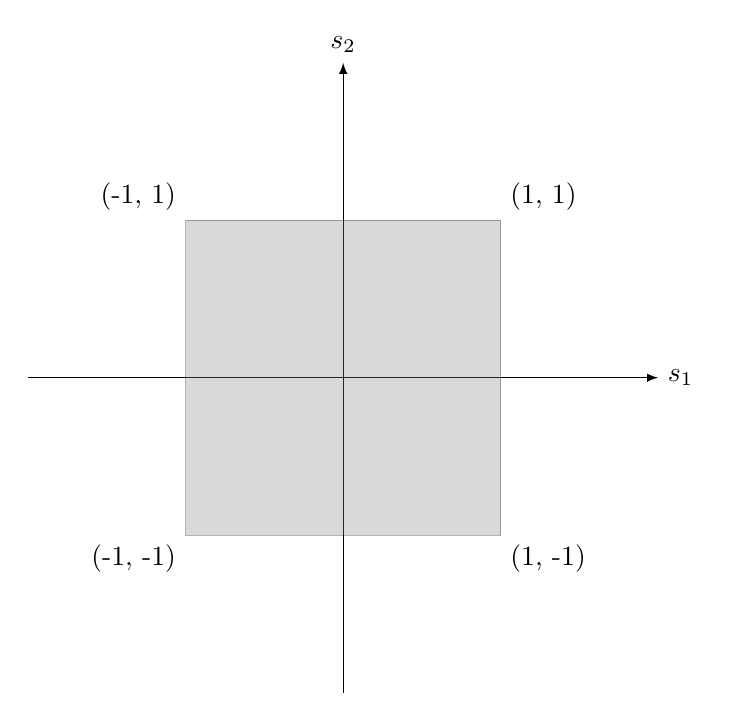
\begin{tikzpicture}
												    
		\draw[-latex] (-4,0) -- (4,0) node[right]{$s_1$};
		\draw[-latex] (0,-4) -- (0,4) node[above]{$s_2$};
													
		\draw [fill=gray, opacity=0.3] (-2,-2) rectangle (2,2);
						
		\draw (-2, -2) node [below left] {(-1, -1)};
		\draw (-2, 2) node [above left] {(-1, 1)};
		\draw (2, -2) node [below right] {(1, -1)};
		\draw (2, 2) node [above right] {(1, 1)};
	\end{tikzpicture}
\end{figure}

\FloatBarrier

Consider the following linear transformation of these signals.

\begin{align*}
	\begin{pmatrix} 
	X_1 \\ 
	X_2 
	\end{pmatrix} & = 
	\begin{pmatrix} 
	1             & 1 \\ 
	1             & 2 
	\end{pmatrix}
	\begin{pmatrix} 
	S_1 \\ 
	S_2
	\end{pmatrix}
\end{align*}

The joint density of the observed signals becomes

\begin{align*}
	P(X_1=x_1,\ X_2=x_2) & = \frac{1}{2\sqrt{5}}\ \ \ if\ (x_1, x_2)\ lie\ in\  parallelogram\ below \\
	                     & = 0\ \ \ otherwise                                                        
\end{align*}


\begin{figure}[htbp]
	\centering
	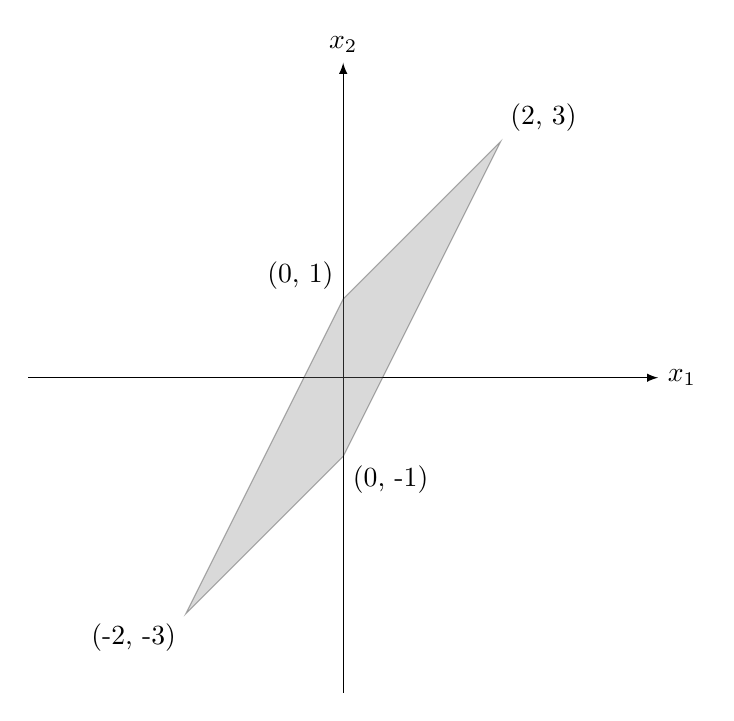
\begin{tikzpicture}
												    
		\draw[-latex] (-4,0) -- (4,0) node[right]{$x_1$};
		\draw[-latex] (0,-4) -- (0,4) node[above]{$x_2$};
													
		\draw [fill=gray,  opacity=0.3] (2,3) -- (0,1) -- (-2,-3) -- (0,-1) -- cycle;
						
		\draw (2, 3) node [above right] {(2, 3)};
		\draw (0, 1) node [above left] {(0, 1)};
		\draw (-2, -3) node [below left] {(-2, -3)};
		\draw (0, -1) node [below right] {(0, -1)};
	\end{tikzpicture}
\end{figure}

\FloatBarrier

One edge of the parallelogram points in the direction $(1, 1)$ and the other in $(1, 2)$. These are the same as the rows in the mixing matrix. This gives some hope that ICA could exploit some properties of the joint distribution to recover the original signals like in this case where the edges of the joint density give the mixing matrix away. 

\section{Relation to PCA}

Given a centered random vector $\boldsymbol{X}$, PCA defines a linear transform $\boldsymbol{Y}\ =\ P \boldsymbol{X}$ such that the resulting vector has uncorrelated components. $P$ is a matrix of orthonormal eigenvectors of the covariance matrix of $\boldsymbol{X}$.

\begin{align*}
	E(\boldsymbol{XX^T}) & = P^TDP 
\end{align*}

The covariance matrix of the transformed random vector is diagonalized.

\begin{align*}
	E(\boldsymbol{YY^T}) & = E(P\boldsymbol{XX^T}P^T) \\
	                     & = PE(\boldsymbol{XX^T})P^T \\
	                     & = PP^TDPP^T                \\
	                     & = D                        
\end{align*}

One can go a step further to define $\boldsymbol{Y}\ =\ D^{-1/2}P\boldsymbol{X}$. Now the covariance matrix of the transformed random vector becomes identity.

\begin{align*}
	E(\boldsymbol{YY^T}) & = D^{-1/2}PE(\boldsymbol{XX^T})P^TD^{-1/2T} \\
	                     & = D^{-1/2}PP^TDPP^TD^{-1/2T}                \\
	                     & = I                                         
\end{align*}

Such a transformation of $\boldsymbol{X}$ is called whitening. Whitening is often a preprocessing step of ICA. Intuitively, whitening makes the transformed components uncorrelated and then ICA will make them independent. So whitening solves half the problem of ICA. More formally, whitening restricts the space of mixing matrix to orthogonal matrices thus making the problem easier. To understand why, consider $\boldsymbol{Y}\ =\  A\boldsymbol{S}$ such that $\boldsymbol{Y}$ is white.

\begin{align*}
	E(\boldsymbol{YY^T}) = I      \\
	AE(\boldsymbol{SS^T}) A^T = I \\
\end{align*}

Since signals are independent with unit variances as per an assumption above,

\begin{align*}
	E(\boldsymbol{SS^T}) & = I \\
	AA^T                 & = I \\
\end{align*}

proving that $A$ must be orthogonal. Hence, in case of a random vector of size $N$, instead of estimating $N^2$ parameters of the matrix $A$, ICA only has to estimate $N(N-1)/2$ parameters since $A$ is orthogonal and an orthogonal matrix has $N(N-1)/2$ degrees of freedom. This is equal to estimating almost half the parameters. Thus, literally too, whitening solves half the problem of ICA.

\section{Why Gaussian signals can't be recovered?}

\section{Algorithm}

\section{Comments}

\end{document}
